\PassOptionsToPackage{unicode,pdfusetitle}{hyperref}
\PassOptionsToPackage{hyphens}{url}
\PassOptionsToPackage{dvipsnames,svgnames,x11names}{xcolor}

\documentclass[10pt,ignorenonframetext]{beamer}

\usepackage{lmodern}
\usepackage{amssymb,amsmath,mathtools,amsthm}
\usepackage[T1]{fontenc}
\usepackage[utf8]{inputenc}
\usepackage{textcomp}

\usepackage{pgfpages}

\usepackage{presentation}

\usepackage{upquote}
\usepackage[]{microtype}
\UseMicrotypeSet[protrusion]{basicmath}

\usepackage{xcolor}
\usepackage{xurl}
\usepackage{bookmark}
\usepackage{hyperref}
\hypersetup{
  colorlinks=true,
  linkcolor=Black,
  filecolor=SteelBlue4,
  citecolor=Orange3,
  urlcolor=SteelBlue4
}

% tikz and pgfplots stuff
\usepackage{tikz}
\usetikzlibrary{arrows,shapes,positioning,intersections,backgrounds}
\usepackage{pgfplots}
\usepgfplotslibrary{external,colormaps}
\pgfplotsset{width=5cm,compat=1.16}
\tikzexternalize[prefix=tikz/]

%\urlstyle{same} % disable mono-spaced font for URLs
\newif\ifbibliography
\setlength{\emergencystretch}{3em} % prevent overfull lines
\setcounter{secnumdepth}{-\maxdimen} % remove section numbering

%\usepackage{subfig}
\usepackage{subcaption}
\usepackage{algorithm,algpseudocode}
\usepackage{booktabs}

% biblatex
\usepackage[style=authoryear]{biblatex}
\addbibresource{references.bib}

\title{Look-Ahead Screening Rules for the Lasso}
\subtitle{EYSM 2021}
\author{Johan Larsson}
\date{\today}
\institute{Department of Statistics, Lund University}
\titlegraphic{
\includegraphics{images/lu-logo.pdf}}

\begin{document}

\frame[plain]{\titlepage}

% \begin{frame}{Overview}
%   \tableofcontents
% \end{frame}

\begin{frame}{The Lasso}
  The lasso~\parencite{tibshirani1996} is a type of penalized regression,
  represented by the following
  convex optimization problem:
  \[
    \operatorname*{minimize}_{\beta \in \mathbb{R}^p}
    \left\{
      P(\beta; \lambda) = \frac 1 2 \lVert y - X\beta \rVert_2^2
      + \lambda \lVert \beta \rVert_1.
    \right\}
  \]

  \begin{columns}[c]
    \begin{column}{0.45\linewidth}
      \(\lambda\) is a hyper-parameter that controls the level of
      \alert{penalization}.
      \medskip\medskip

      \(\hat\beta_\lambda\) is the solution to this problem for a given
      \(\lambda.\)

    \end{column}
    \begin{column}{0.45\linewidth}
      \begin{figure}
        \centering
        \pgfplotsset{width=6cm,height=6cm}
        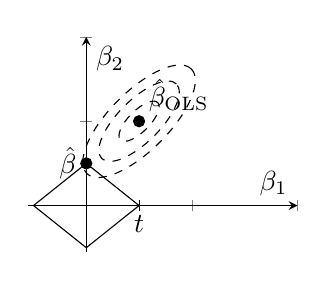
\begin{tikzpicture}
\begin{axis}[
    xlabel = \(\beta_1\),
    ylabel = \(\beta_2\),
    ymin = -1.1,
    ymax = 4,
    xmin = -1.1,
    xmax = 4,
    axis lines = center,
    yticklabels={,,},
    xticklabels={,,}
]
\draw[dashed, rotate around={45:(1,2)}] (1,2) ellipse (0.5 and 0.25);
\draw[dashed, rotate around={45:(1,2)}] (1,2) ellipse (1 and 0.5);
\draw[dashed, rotate around={45:(1,2)}] (1,2) ellipse (1.4 and 0.7);

\addplot[]
    coordinates {
    	(-1,0)
    	(0,1)
    	(1,0)
    	(0,-1)
    	(-1,0)
    };
    
\addplot [only marks, mark=*] coordinates {(1,2)};
\node [above right,black] at (1,2) {\(\hat\beta_\text{OLS}\)};

\addplot [only marks, mark=*] coordinates { (0,1) };
\node [left] at (0,1) {$\hat\beta$};

\addplot [only marks, mark = |] coordinates { (1, 0) };
\node [below] at (1,0) {\(t\)};
\end{axis}
\end{tikzpicture}
      \end{figure}
    \end{column}
  \end{columns}


\end{frame}

\begin{frame}{The Lasso Path}
  \begin{figure}
    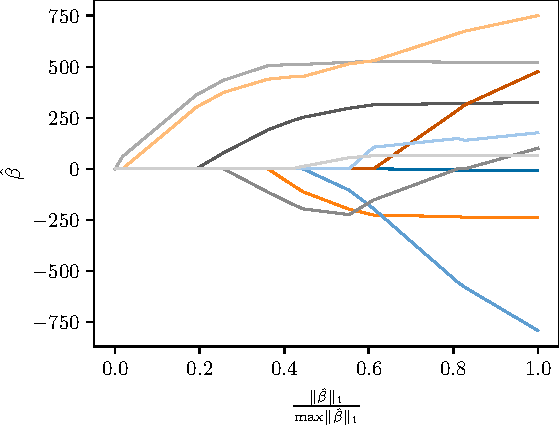
\includegraphics{images/lasso-path}
  \end{figure}
\end{frame}

\begin{frame}{Predictor Screening Rules}
  \begin{block}{motivation}
    Many of the solution vectors, \(\hat\beta\),
    along the regularization path will be \alert{sparse}, which means some
    predictors (columns) in \(X\) will be \alert{inactive}, especially
    if \(p \gg n\).
  \end{block}
  \pause
  \begin{block}{basic idea}
    If we could, based on a relatively \alert{cheap} test, determine which
    predictors will be inactive before fitting the model, we could solve
    the problem \alert{much faster}. 	
  \end{block}
  \pause
  \begin{block}{it turns out we can!}
    using screening rules
  \end{block}
\end{frame}

\begin{frame}[c]
  \frametitle{The Dual}
  The \alert{dual} is a complementary problem to the primal problem.
  For the lasso, it is
  \[
    \operatorname*{maximize}_{\theta \in \mathbb{R}^n}
    \Big\{
    D(\theta; \lambda) = \frac 1 2 y^T y -
    \frac{\lambda^2}{2} \Big\lVert \theta - \frac y \lambda \Big\rVert_2^2.
    \Big\}
  \]
  \begin{columns}
    \begin{column}[t]{0.45\linewidth}
      The \alert{duality gap} is the difference between the primal and dual
      objectives and is tight at the optimum, that is
      \[
        P(\hat\beta; \lambda) - D(\hat\theta; \lambda) = 0.
      \]
    \end{column}
    \begin{column}[t]{0.45\linewidth}
      \begin{figure}[htpb]
        \centering
        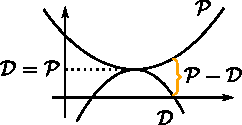
\includegraphics[]{images/duality-gap.pdf}
        % \caption{Duality }%
        \label{fig:images/duality-gap}
      \end{figure}
    \end{column}
  \end{columns}
  \medskip
  \medskip

  This means that the dual and primal---in the case of the lasso---are related
  via
  \[
    y = X\hat\beta(\lambda) + \lambda \hat \theta(\lambda).
  \]
\end{frame}

\begin{frame}[c]
  \frametitle{KKT Conditions}
  The Karush--Kuhn--Tucker (KKT) stationarity condition for the lasso specify
  that
  \[
    \boldsymbol{0} \in X^T(X\beta - y) + \lambda\partial,
  \]
  where \(\partial\) is the subdifferential of the \(\ell_1\) norm, with
  elements given by
  \[
    \partial_j  =
    \begin{cases}
      \{\sign(\hat\beta_j)\} & \text{if }\hat\beta_j \neq 0 \\
      [-1,1]                 & \text{if } \hat\beta_j = 0.
    \end{cases}
  \]
  This means that \[
    |x_j^T \hat\theta| < 1 \implies \hat\beta_j = 0.
  \]
\end{frame}

\begin{frame}[c]
  \frametitle{Safe Screening Rules}
  Safe screening rules work by finding a region within which the dual-optimal
  solution, \(\hat\theta\), must lie.
  \medskip

  \begin{figure}[htpb]
    \centering
    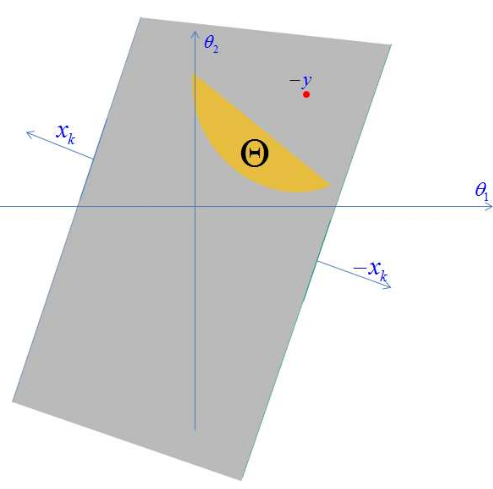
\includegraphics[height=4cm]{images/safe-regions.png}
    \caption{Safe region from original SAFE screening rule.}%
    \label{fig:safe-regions}
  \end{figure}

  I.e., we replace the inequality \(|x_j^T \hat\theta| < 1\) with an inequality
  that leads to the same conclusion, but doesn't involve \(\hat\theta\).
\end{frame}

\begin{frame}[c]
  \frametitle{Gap Safe Screening Rule}
  The Gap Safe screening rule uses the \emph{duality gap} to define such a
  region, and disards the \(j\)th predictor if
  \begin{equation*}
    |X^T \theta_\lambda|_j + \lVert x_j\rVert_2
    \sqrt{
      \frac{1}{\lambda_*^2}
      \big(\mathcal{P}(\beta_\lambda; \lambda^*) -
      \mathcal{D}(\theta_\lambda; \lambda^*)\big)
    }
    < 1
  \end{equation*}
  where
  \[
    \theta_\lambda = \frac{y - X\beta_\lambda}{
      \max\big( |X^T(y - X\beta_\lambda)|, \lambda\big)}.
  \]
  \medskip

  \begin{block}{Dynamic Screening}
    Duality gap \emph{decreases} during iterative
    optimization---screening becomes better and better.
  \end{block}
\end{frame}

\begin{frame}[c]
  \frametitle{Our Contribution: Look-Ahead Screening}
  Inequality on last slide is \emph{quadratic}, which means we can find the next
  \emph{critical} point easily:
  \[
    \lambda_* = \frac{-b \pm \sqrt{b^2 - 4ac}}{2a} \quad
  \]
  where
  \[
    \begin{aligned}
      a & = \big( 1 - | x_j^T \theta_\lambda|\big)^2 -
      \frac 12 \theta_\lambda^T \theta_\lambda \lVert x_j\rVert_2^2,     \\
      b & = \big(\theta_\lambda^T y - \lVert \beta_\lambda \rVert_1\big)
      \lVert x_j \rVert_2^2,                                             \\
      c & = - \frac 12 \lVert y - X\beta_\lambda\rVert_2^2
      \lVert x_j\rVert_2^2.                                              \\
    \end{aligned}
  \]
  This allows us to screen predictors for all upcoming steps.
  \medskip

  \pause

  Say we are at step \(k\) along the path; then simply check the inequality for
  all \(\lambda_{k +1},\lambda_{k + 2}, \dots\)
\end{frame}

\begin{frame}[c]
  \frametitle{Example}

  \begin{figure}
    \centering
    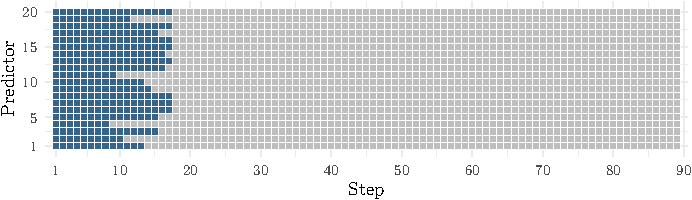
\includegraphics[width=\textwidth]{images/casestudy.pdf}
    \caption{The predictors screened at the first step of the
      lasso path via look-ahead screening for a random sample of
      20 predictors from the \emph{leukemia}
      data set. A blue square indicates that the corresponding predictor can
      be discarded at the respective step.\label{fig:case-study}}
  \end{figure}

\end{frame}

\begin{frame}[c]
  \frametitle{Results on Simulated Data}
  \begin{figure}[hbtp]
    \centering
    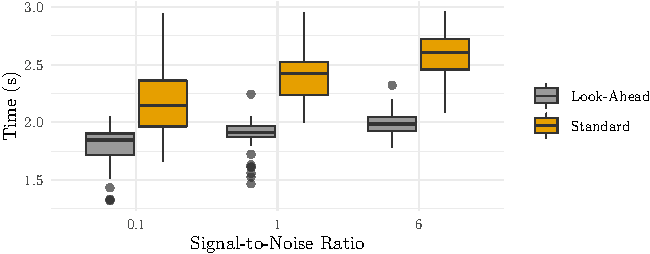
\includegraphics[width=\textwidth]{images/simulated-data-timings.pdf}
    \caption{Standard box plots of timings to fit a full lasso path to
      a simulated data set with \(n = 100\), \(p = 50\,000\), and five
      true
      signals.}
    \label{fig:simulated-data}
  \end{figure}

  code and results available at
  \href{https://github.com/jolars/LookAheadScreening}{github.com/jolars/LookAheadScreening} 
\end{frame}

\begin{frame}[c]
  \frametitle{Conclusions}
  \begin{itemize}
    \item simple idea; easily extendable to other rules with similar properties
    \item application comes essentially \emph{for free}
    \item agnostic to solver used
    \item likely works for other loss function too (but we have not studied this
          yet)
  \end{itemize}
\end{frame}

\begin{frame}[allowframebreaks]{References}
  \bibliographytrue
  \printbibliography[heading=none]
\end{frame}


\end{document}
